\documentclass{article}
\title{Apuntes de códigos bloque lineales y cíclicos. FEC y ARQ}
\author{Eugenio Cano Muñoz\\ G31 - ETSIT UPM}
\date{Curso 2023 - 2024}


\usepackage{tikz}
\usetikzlibrary{positioning, shapes, shapes.arrows}

\tikzstyle{block} = [draw, rectangle, 
    minimum height=3em, minimum width=6em]
\tikzstyle{pinstyle} = [pin edge={to-,thin,black}]

\usepackage{amssymb}
\usepackage{amsmath}
\usepackage{circuitikz}
\usepackage{xfrac}

\begin{document}
\maketitle

\pagebreak

This work is licensed under CC BY-NC 4.0. To view a copy of this license, visit http://creativecommons.org/licenses/by-nc/4.0/

\pagebreak

\section{Códigos de fuente}

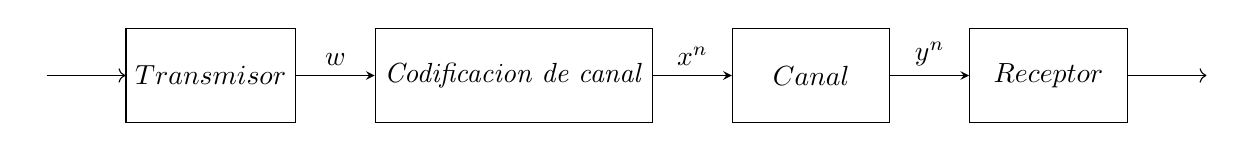
\begin{tikzpicture}
    \node[](input){};

    \node[
        draw,
        minimum width=2cm,
        minimum height=1.2cm,
        right=1cm of input] (Tx) {$Transmisor$};
    \node[
        draw,
        minimum width=2cm,
        minimum height=1.2cm,
        right=1cm of Tx] (CC) {\textit{Codificacion de canal}};
    \node[
        draw,
        minimum width=2cm,
        minimum height=1.2cm,
        right=1cm of CC] (Canal) {$Canal$};
    \node[
        draw,
        minimum width=2cm,
        minimum height=1.2cm,
        right=1cm of Canal] (Rx) {$Receptor$};

    \node[right=1cm of Rx](output) {};

    \draw[-stealth] (Tx.east) -- (CC.west)
    node[midway,above]{$w$};
    \draw[-stealth] (CC.east) -- (Canal.west)
    node[midway,above]{$x^n$};
    \draw[-stealth] (Canal.east) -- (Rx.west)
    node[midway,above]{$y^n$};

    \draw[draw, ->] (input) -- (Tx.west)
    node[midway,above]{};
    \draw[draw, ->] (Rx.east) -- (output)
    node[midway,above]{};
\end{tikzpicture}

\subsection{Repaso de Álgebra binaria}

Tenemos un alfabeto formado por $\{0,1\}$ y las siguientes operaciones $\oplus$ (suma) y $\odot$ (multiplicación):

\begin{center}
     \begin{tabular}{|c|c|c|}
        \hline
           $\oplus$ & 0 & 1 \\
        \hline
            0 & 0 & 1 \\
        \hline
            1 & 1 & 1 \\
        \hline
    \end{tabular}
    \begin{tabular}{|c|c|c|}
        \hline
           $\odot$ & 0 & 1 \\
        \hline
            0 & 0 & 1 \\
        \hline
            1 & 0 & 1 \\
        \hline
    \end{tabular}
\end{center}

\subsubsection{Cuerpo de Galois:}

Es un \textbf{grupo} - Sea g un conjunto de elementos:
\begin{enumerate}
    \item Tiene una operación binaria
    \item Esta asociación binaria es asociativa
    \begin{equation}
        a \circledast (b \circledast c) = (a \circledast b) \circledast c
    \end{equation}
    \item Existe un elemento neutro tal que
    \begin{equation}
        \begin{split}
        \exists e \in G;\exists a \in G \\
        a \circledast e= e \circledast a = a
        \end{split}
    \end{equation}
    \item Todo elemento de un grupo tiene su inverso
    \begin{equation}
        \begin{split}
            \forall a \in G; \exists a' \in G \\ 
            a \circledast a' \in e
        \end{split}
    \end{equation}
\end{enumerate}
G es un \textbf{grupo conmutativo} si:

\begin{enumerate}
    \item G es un grupo
    \item se cumple la propiedad conmutativa:
    \begin{equation}
        a \circledast b = b \circledast a
    \end{equation}
\end{enumerate}
F es un \textbf{grupo con dos operaciones} $\oplus$ y $\odot$ si:

\begin{enumerate}
    \item F es un grupo conmutativo bajo $\cdot$
    \item El 4º elemento $\neq e$ del F es un grupo conmutativo bajo $\cdot$
    \item La multiplicación des tristributiva bajo la condición:
    \begin{equation}
        a \cdot (b + c) = a \cdot b + a \cdot c
    \end{equation}
\end{enumerate}

Si el alfabeto es finito $\Rightarrow$ Cuerpo de Galois ($GF(n)$), siendo n la longitud del alfabeto

\begin{enumerate}
    \item El conjunto $\forall n$ tomando $(v_1, v_2, ..., v_n), v_i\in GF(2)$ junto con las operaciones:
    \begin{equation}
        \begin{split}
            +: \vec{u} + \vec{v} = \vec{w}; w_i = u_i +v_i \\
            \cdot: = \lambda \cdot \vec{u}=\vec{w}; w_i=\lambda b_i
        \end{split}
    \end{equation}
    es un espacio vectorial sobre sobre $GF(2)$     
    \item $\mathcal{S} \subseteq V_n$ es un subespacio vectorial si:
    \begin{enumerate}
        \item $\varnothing \in \mathcal{S}$
        \item $\forall \vec{u}, \vec{v}\in \mathcal{S}, (\vec{u} + \vec{v}) \in \mathcal{S}$
        \item $(\lambda\cdot\vec{u})\in \mathcal{S}$
    \end{enumerate}
    \item Dato $\vec{v_1}, \vec{v_2}, ..., \vec{v_n}$ se dice que son linealmente independientes si $\forall c_i \Rightarrow c_1\vec{v_1} + c_2\vec{v_2} + .. + c_n\vec{v_n} \neq 0$ excepto $c_1 = c_2 = ... = c_n = 0$
    \item El conjunto $\{\vec{g_1}, \vec{g_2}, ..., \vec{g_n\}}$ genera $V_n$ si $\forall v \in V_n \Rightarrow \vec{v} = \sum_{i=1}^{n}{c_i\vec{g_i}}$
    \item En todo $V_n, \exists\{\vec{g_1}, \vec{g_2}, ..., \vec{g_n}\}$ linealmente independientes que generan $V_n$ (Su cardinal es $n$)
    \item Si $K < n; \{\vec{v_1}, \vec{v_2}, ... \vec{v_k}\}\subseteq V_n$ es un subespacio vectorial de dimensión $K$
    \item Se define el operador del producto interior $\vec{u} \cdot \vec{v} = u_1v_1+u_2v_2+....+u_nv_n$
    \item Se dice que $\vec{u}$ y $\vec{v}$ son ortogonales si $\vec{u}\cdot\vec{v} = 0$
    \item Sea $\mathcal{S}$ un subespacio vectorial de dimensión $k\subseteq V_n$. Sea $\mathcal{S}_d$ el conjunto de vectores $\subseteq V_n / \forall \vec{u} \in \mathcal{S}; \forall \vec{v} \in \mathcal{S}_d \Rightarrow \vec{u} \cdot \vec{v}=0$ $\mathcal{S} \equiv$ Espacio dual de $\mathcal{S}$ dimensión $(n \cdot k)$

\end{enumerate}

\pagebreak
\subsection{Códigos lineales}

\textbf{Código:} Transformación de una palabra $k$ bits a $n$ bits.

\begin{equation}
    \mathcal{C}(n,k)
\end{equation}

\begin{enumerate}
    \item Códigos
    \begin{enumerate}
        \item lineales
        \begin{enumerate}
            \item Bloque
            \begin{enumerate}
                \item Cíclicos
                \item No cíclicos
            \end{enumerate}
            \begin{enumerate}
                \item Sistemáticos
                \item No sistemáticos
            \end{enumerate}
            \item Convolucionales
        \end{enumerate}
        \item No lineales
    \end{enumerate}
\end{enumerate}

\paragraph{Código bloque:} Los datos se dividen en bloques binarios de tamaño $k$, llamados bits de mensaje. Cada bloque puede representar uno de los $2^k$ mensajes distintos. El codificador transforma la palabra de $k$ bits a otra de $n$ bits. Los bits $r=(n-k)$ se denominan \textbf{bits reduntantes} o \textbf{bits de paridad}, ya que no aportan nueva información. El \textbf{radio de redundancia del código} es la relación de bits redundantes a bits de mensaje y se puede obtener de la siguiente forma $(n-k)/k$. La \textbf{tasa del código} es $k/n$, que se puede explicar como la porción del código que aporta información.

\paragraph{Código lineal:} Son una clase de códigos que pueden ser caracterizados por la notación $(n,k)$ ya mencionada. El codificador transforma un bloque de $k$ bits en uno de $n$ bits (aunque en este texto siempre se hable de bits, también es posible utilizar otro tipo de alfabetos). Los diferentes $2^k$ mensajes se denominan las \textbf{k-tuplas}, y los $2^n$ mensajes se denominan las \textbf{n-tuplas}. El proceso de codificación asigna una k-tupla a cada una de las n-tuplas de forma biyectiva. Esta asignación es lineal para códigos lineales.

\pagebreak

\subsubsection{Matriz generadora:} 

Como las palabras código que forman un bloque lineal, es un subespacio vectorial de dimensión $k$ del espacio vectorial de dimensión $n$ ($k<n$), utilizar un conjunto de vectores generadores para "expandir" el subespacio. La combinación linealmente independiente más pequeña que expande el subespacio se denomina la \textbf{base generadora} del subespacio, y el número de vectores en esta basa es la dimensión del subespacio ($k$). En general, definimos la matriz generadora como la siguiente matriz de tamaño $k \times n$:

\begin{equation}
    \begin{split}
        \vec{v} = (v_0, v_1, ... v_{n-1}); \vec{u} = (u_0, u_1, ..., u_{n-1}) \\
       \vec{v}=\vec{u}
       \begin{pmatrix}
            g_{00} & g_{01} & ... & g_{0,n-1} \\
            g_{10} & g_{11} & ... & g_{1,n-1} \\
            ... & ... & ... & ... \\
            g_{k-1,0} & g_{k-1, 1} & ... & g_{k-1, n-1}
       \end{pmatrix} 
    \end{split}
\end{equation}

En esta ecuación, podemos ver que el vector $\vec{u}$ son las palabras código del subespacio vectorial $n$ y $\vec{v}$ son las palabras del espacio vectorial $k$. La operación anterior también se puede representar como:

\begin{equation}
    \vec{v} = \vec{u}G
\end{equation}

Como podemos ver, la matriz G, está formada por los vectores código, que se establecen como vectores en filas.

\begin{equation}
    G = 
    \left(
        \begin{array}{c}
            \vec{v_0} \\
            \vec{v_1} \\
            ... \\
            \vec{v_{k-1}}
        \end{array}
    \right)
\end{equation}

\subsubsection{Estructuración sistemática:} 

Los códigos sistemáticos es una relación entre un vector mensaje $k$-dimensional y un una palabra código $n$-dimensional, de tal forma que parte de la secuencia generada coincida con los bits $k$ del mensaje, los bits $n-k$ son bits de paridad. Los bloques de códificación sistemática tienen una matriz generadora de la siguiente forma:

\begin{equation}
    G_s(p|I_c) =
    \left(
        \begin{array}{cccc|cccc}
            p_{0,0} & p_{0,1} & ... & p_{0, n-k-1} & 1 & 0 & ...  & 0 \\
            p_{1,0} & p_{1,1} & ... & p_{1, n-k-1} & 0 & 1 & ...  & 0 \\
            ... & ... & ... & ... & ... & ... & ...  & ... \\
            p_{k-1,0} & p_{k-1,1} & ... & p_{k-1, n-k-1} & 0 & 0 & ...  & 1 \\
        \end{array}
    \right)
\end{equation}

En este caso, $p$ es la porción de paridad de la matriz generadora e $I_c$ es la matriz identidad $k\times k$. En la Estructuración sistematica no hace falta guardar la parte de la matriz iddentidad, podemos entonces entender que código $\mathcal{C}(n,k)$ como $\mathcal{C}(k+paridad,k)$

Otra forma válida de establecer la matriz generadora sistemática $G_s$, podría ser para que los bits del mensaje ocupasen la parte izquierda y los bits de paridad la parte derecha, generando la matriz $G(I_c|p)$

\subsubsection{Matriz de comprobación de paridad $(H)$:} 

La matriz de comprobación de paridad $H$ nos permitirá decodificar los vectores recibidos. Todas las matrices generadoras $G$ tienen una matriz $H$ de tamaño $(n-k)\times n$, de tal forma que las filas de $G$ sean ortogonales a las filas de $H$, osea que $GH^T = 0$. Partiendo de las estructuración sistemática, podemos general la matriz de paridad de una forma sencilla, estableciendo una matriz identidad de tamaño $(n-k)$ en la parte izquierda y la submatriz de paridad transpuesta $p^t$ que obtenemos de la matriz generadora $G$, dicho de otra forma:

\begin{equation}
    G_s = (p|I_k) \to H(I_{n-k}|p^t)
\end{equation}

por lo que la matriz de comprobación de paridad transpuesta $H^T$ resultaría de la siguiente forma

\begin{equation}
    H^T =
    \left(
        \begin{array}{c}
            I_{n-k} \\
            \hline \\
            P 
        \end{array}
    \right)
\end{equation}

Por lo tanto, si tenemos una cadena codificada $\vec{r}$ que ha pasado por el canal, podemos saber si esta pertenece al código si al multiplicarla por la matriz de comprobación de paridad transpuesta resulta en un vector $\vec{0}$, en caso contrario, la palabra ha sido alterada por el canal y la palabra no pertenece al código:

\begin{equation}
    \vec{r} \to \vec{r}\cdot H^t =
    \left\{
        \begin{array}{c}
           = 0 \Rightarrow \vec{r} \in \mathcal{C} \\
           \neq 0 \Rightarrow \vec{r} \notin \mathcal{C}
        \end{array}
    \right\}
\end{equation}

\subsubsection{Síndrome:}

Si $\vec{r}$ es el vector resultante de la transmisión por un canal del vector $\vec{u}$, podemos describir el vector recibido como:

\begin{equation}
    \vec{r} = \vec{v} + \vec{e}
\end{equation}

O con notación de bloques:

\begin{center}
    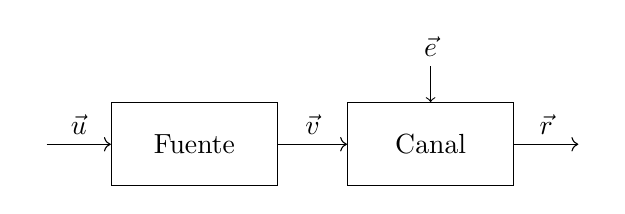
\begin{tikzpicture}[auto, node distance=2cm]
        \node[](in){};

        \node[
            block,
            right of=in
        ](fuente){Fuente};

        \node[
            block,
            right of=fuente,
            pin={[pinstyle]above:$\vec{e}$},
            node distance=3cm
        ](canal){Canal};

        \node[right of=canal](out){};

        \draw[->] (in) -- node {$\vec{u}$} (fuente);
        \draw[->] (fuente) -- node {$\vec{v}$} (canal);
        \draw[->] (canal) -- node {$\vec{r}$} (out);
    \end{tikzpicture}   
\end{center}

En donde que vector error $\vec{e} = (e_0, e_1, ... e_n)$ se define de la siguiente forma:

\begin{equation}
    e_i = 
    \left\{
        \begin{array}{c}
           0 \Rightarrow \text{No afecta bit } i \\
           1 \Rightarrow \text{Error en bit } i 
        \end{array}
    \right\}
\end{equation}


\pagebreak

$\vec{e}$ es un vector de error introducido por el canal. Extisten un total de $2^n-1$ Posibles errores en un espacio de $2^n$. Para detectarlos, definimos el síndrome de $\vec{r}$:

\begin{equation}
    \vec{S} = \vec{r} H^t = 
    \left\{
        \begin{array}{c}
           = 0 (\vec{r} \in \mathcal{C}) \\
           \neq 0 (\vec{r} \notin \mathcal{C}) 
        \end{array}
    \right\}
\end{equation}

El síndrome es el resultado de la comprobación de paridad realizada a $\vec{r}$ para determinar si es un miembtro válido del conjunto de palabras código. Si $\vec{r}$ es un miembro, el síndrome $S$ es igual a cero, y si contiene errores detectables, tiene cualquier otro valor que muestra el patrón de error. Posterior mente el codificador intentará corregir el error o pedirá una segunda transmisión. Combinando las ecuaciones anteriores:

\begin{equation}
    \vec{S} = \vec{r} H^t = (\vec{v} + \vec{e}) H^t = (\vec{v} H^t)|_{= 0} + \vec{e}H^t = \vec{e}H^t
\end{equation}

Una característica importante de los códigos bloque lineales es que la relación entre los patrones de errores corregibles y el síndrome es uno a uno..

Además hay que añadir dos requisitos a la matriz de comprobación de paridad:

\begin{enumerate}
    \item Ninguna columna de la matriz de comprobación de paridad puede contener todo ceros, sino un error en la palabra código correspondiente no podría afectar al síndrome y sería indetectable
    \item Todas las columnas de la matriz de comprobación deben ser distintas. Si dos columnas de la matriz fuesen idénticas, no se podrían percibir errores en las posiciones de las palabras código
\end{enumerate}

En el caso en el que el producto $\vec{r}H^t = \vec{0}$, podemos tener dos posibilidades, que $\vec{e} = \vec{0}$, es decir, que no haya un error o $\vec{e} \neq \vec{0}$ o que haya un error indeterminado, es por eso que se desea evitar que $\exists \vec{e} \in \mathcal{C}, \forall \mathcal{C} \Rightarrow \vec{v}$ tenga muchos 1s, si la probabilidad de error es menor que 0,5 ($p_e < 0.5$)

\pagebreak

\subsubsection{Corrección de errores y tabla estándar:} 

A partir del síndrome no solo podemos detectar el patrón de error, sino que podemos corregirlo, ya que existe una correspondencia bit a bit. Si representamos todas las $2^n$ n-tuplas que representan los vectores posiblemente recividos en una matriz, llamada la \textbf{tabla estándar}, tal que la primera fila contenga todas las palabras código empezando por la palabra código $\vec{0}$ y la primera columna contenga todos los posibles patrones de error corregibles. En esta tabla el resto de filas reciben el nombre de \textit{cogrupo}. La primera columna de la fila recibe el nombre de \textit{líder de cogrupo}, seguida de las palabras alteradas por dicho patrón de error, quedando dicha tabla de la siguiente forma:

\begin{equation}
    \left\{
        \begin{array}{cccccc}
            \vec{v_0} & \vec{v_1} & ... & \vec{v_i} & ... & \vec{v_{2^{(k-1)}}} \\
            \vec{e_1} & \vec{e_1} + \vec{v_1} & ... & \vec{e_1} + \vec{v_i} & ... & \vec{e_1} + \vec{v_{2^{(k-1)}}}  \\
            ... & ... & ... & ... & ... & ... \\
            \vec{e_{n-k}} & \vec{e_{n-k-1}} + \vec{v_1} & ... & \vec{e_{2^{n-k-1}}}+\vec{e_1} & ... & \vec{e_{n-k-1}} + \vec{v_{2^{k-1}}}
        \end{array}
    \right\}
\end{equation}

Como se ha mencionado antes, la creación de la matriz se realiza de la siguiente forma:

1ª Fila: códigos definidos dentro del código:

\begin{equation}
    \vec{v_i} \in \mathcal{C}
    \left\{
        \begin{array}{c}
            \vec{v_0} = \vec{0} \\
            \vec{v_i}
        \end{array}
    \right.
\end{equation}

Resto de filas: la primera columna es un vector de error y las siguientes son el código más el error:

\begin{equation}
    \vec{v_i} \notin \mathcal{C}
    \left\{
        \begin{array}{c}
            \vec{e_1} \Rightarrow \text{1ª columna} \\
            \vec{e_j} + \vec{v_i} \Rightarrow \text{Demás columnas}
        \end{array}
    \right.
\end{equation}

El término cogrupo en este caso se utiliza para denominar un grupo de números que comparten una característica común, en este caso, se puede apreciar a primera vista que cada miembro del cogrupo tienen el mismo grupo. Este síndrome lo utilizamos para detectar el patrón de error. Podemos demostrar lo dicho anteriormente de la siguiente forma:

\begin{equation}
    \left\{
        \begin{array}{c}
            \vec{v_i} + \vec{e_j} \Rightarrow \vec{s_i} = (\vec{v_i} + \vec{e_j})H^t = \vec{e_j}H^t \\
            \vec{v_k} + \vec{e_j} \Rightarrow \vec{s_k} = (\vec{v_i} + \vec{e_j})H^t = \vec{e_j}H^t \\
        \end{array}
        \Rightarrow \text{mismo síndrome}
    \right.
\end{equation}

Partiendo de esto, con el vector síndrome, podemos calcular el error del código, detectarlo y corregirlo de la siguiente forma:

\begin{enumerate}
    \item Calculamos el síndrome de $\vec{r}$ utilizando la ecuación $\vec{s} = \vec{r}H$.
    \item Identificar el líder del cogrupo con el mismo síndrome $\vec{s}$. Este patrón de error será considerada la perturbación introducida por el canal.
    \item La palabra código corregida se identifica como $\vec{v} = \vec{r} + \vec{e}$ (En álgebra binaria la resta es idéntica a la suma).
\end{enumerate}

La tabla estandar contiene todas las $2^n$ entradas en el espacio de n-tuplas, sin nada repetido. Al principio puede parecer que esta herramienta se limita a bloques código pequeños, pero la tabla estandar nos permite la visualización de problemas de rendimiento hasta en códigos grandes, como compromisos entre corrección de erreores y detección.

El número de coeficientes $\alpha$ de peso $i$ ($\alpha_i$) se puede calcular de la siguiente forma:

\begin{equation}
    \alpha_i =
    \left(
    \begin{array}{c}
       n\\
       i 
    \end{array}
    \right)
\end{equation}

Estos coeficientes rellenarán la tabla estándar hasta completarla. Como ya se expuso antes, la tabla tiene una \textbf{capacidad} de $2^n$ entradas, con $2^k$ columnas y $2^{n-k}$ filas. En un \textbf{código perfecto}, los líderes de cogrupo deben ser todos los vectores menores a un determinado peso y ninguno más.

A pesar de que existen metodos de corrección, se tienen que cumplir ciertas condiciones para poder corregir un código.

\subsubsection{Pesos y distancias de hamming:}

Dado una palabra código $\vec{v}$ procedente de un código lineal $\mathcal{C}(n,k)$ podemos definir distintos parámetros que nos servirán a la hora de determinar las condiciones de corrección de un código.

El \textbf{Peso de Hamming de v ($\omega (\vec{v})$)} es el número de elementos no nulos en $\vec{v}$ (o dicho de otra forma el número de unos dentro de la palabra código).

La \textbf{Distancia de Hamming entre $\vec{v} \times \vec{w}$ ($d(\vec{v}, \vec{w})$)} es el número de bits que diferencian las palabras código $\vec{v}$ y $\vec{w}$. Cabe recalcar que en este caso también se cumple la desigualdad triangular:
\begin{equation}
    d(\vec{v}, \vec{w}) + d(\vec{w}, \vec{x}) \geq d(\vec{v}, \vec{x})
\end{equation}

De lo anterior podemos apreciar que la distancia de Hamming entre dos vectores es igual al peso de la suma de los vectores, ya que de esta forma, los elementos idénticos se anularán

\begin{equation}
    d(\vec{v}, \vec{w}) = \omega(\vec{v}+\vec{w})
\end{equation}

Considere el conjunto de distancias entre todas las palabras código en el espacio vectorial. La \textbf{distancia mínima de un código $d_{min}$} es la mínima distancia de hamming en un código, esta distancia representa la parte más débil frente a errores del código, y por eso caracteriza la robustez del código.

\begin{equation}
    d_{min} = min\{d(\vec{v},\vec{w});\vec{v},\vec{w}\in\mathcal{C};\vec{v}\neq\vec{w}\} = min\{\omega(\vec{v}+\vec{w});\vec{v},\vec{w}\in\mathcal{C};\vec{v}\neq\vec{w})\}
\end{equation}

Para calcular la distancia mínima, tenemos que tener en cuenta que las palabras código son cualquiera de las palabras generadas a partir de las palabras código, por lo que hay que calcular la distancia de hamming entre todas las palabras resultantes de $\vec{w_{ij}} = \vec{u_i} + \vec{v_j}$. Para evitar todo este trabajo, tenemos varios mecanismos para calcular esta distancia mínima:

\begin{enumerate}
    \item \textbf{$d_{min} = 0$} Una columna contiene todo ceros
    \item \textbf{$d_{min} = 1$} Dos columnas iguales
    \item \textbf{$d_{min} = 2$} Dos columnas suman 0
    \item \textbf{$d_{min} = n$} n columnas suman 0
\end{enumerate}

\subsubsection{Capacidad de detección:}

La tarea de un decodificador óptimo es asignar la palabra código más probable al mensaje recibido por el canal (teniendo en cuenta que el canal va a insertar errores).

\begin{equation}
    max\{p\} \left\{
    \begin{array}{c}
        \vec{e_0} = \vec{r} + \vec{v_0} \\
        \vec{e_1} = \vec{r} + \vec{v_1} \\
        ... \\
        \vec{e_{L-1}} = \vec{r} + \vec{v_{L-1}} 
    \end{array}
    \right.
\end{equation}

Debemos escoger $\vec{e_i}$ tal que:

\begin{equation}
    min\{\omega(\vec{e_i})\}=
    min\{\omega(\vec{r}+\vec{v_i})\}=
    min\{d(\vec{v},\vec{r})\}
\end{equation}

Sabiendo como funciona el decodificador óptimo, podemos concluir que no siempre va a recuperar la palabra correcta. Llegado a una cierta distancia de Hamming, podemos encontrar otras palabras código válidas, por lo que puede que no tengamos errores detectables, sabiendo esto, podemos concluir que la máxima distancia de corrección $S$ es:

\begin{equation}
    S = d_{min} - 1
\end{equation}

La \textbf{Probabilidad de error} es la probabilidad de que ciertos bits hayan sido alterados y no se pueda recibir la palabra código original. 

\begin{center}
    \begin{tikzpicture}[auto, node distance=2cm]
        \node[](in){};

        \node[
            block,
            right of=in,
            pin={[pinstyle]above:$\vec{e}$},
            node distance=3cm
        ](canal){Canal};

        \node[right of=canal](out){};

        \draw[->] (in) -- node {$\vec{v}$} (canal);
        \draw[->] (canal) -- node {$\vec{r}$} (out);
    \end{tikzpicture}
\end{center}

Para calcular las probabilidades de detección de errores, establecemos $p$ como la probabilidad de que ocurra un cambio de bit en el canal $(1-p)$ como la de que no ocurra, a partir de esto pa partir de esto podemos establecer la probabilidad de error del código para un peso de Hamming \textit{mayor} o igual que $L$, podemos seguir la siguiente ecuación:

\begin{equation}
    P(\omega (e) \geq L ) = \sum_{i=L}^{N}
    \left(\begin{array}{c}
        n \\
        i    
    \end{array}\right)
    p^i(1-p)^{n-i}
\end{equation}

\pagebreak

y la probabilidad de que el error sea \textit{menor} que el peso de Hamming (incluyendo una transmisión correcta de la información):

\begin{equation}
    P(\omega (e) < L ) = \sum_{i=0}^{L-1}
    \left(\begin{array}{c}
        n \\
        i    
    \end{array}\right)
    p^i(1-p)^{n-i}
\end{equation}

Distribución de pesos de palabras código $A_i$ es el número de palabras código que pesan $i$. Con esto se puede hacer un histograma con el que representar la distribución de probabilidades.

La \textbf{probabilidad de error indetectable} es la probabilidad de que haya un error que no pueda ser detectado:

\begin{equation}
    P_{ND} = \sum_{i=d_{min}}^{n}A_ip^i(1-p)^{n-i}
\end{equation}

Si no se conoce la distribución $A_i$, para calcular $P_{ND}$, o calcularla es demasiado complicado, podemos obtener una cota superior:

\begin{equation}
    P_{ND} = \sum_{i=d_{min}}^{n}A_ip^i(1-p)^{n-i} \leq \sum_{i=d_{min}}^{L-1}
    \left(\begin{array}{c}
        n \\
        i    
    \end{array}\right)
    p^i(1-p)^{n-i}
\end{equation}

Si queremos hacer una aproximación mas burda de esta probabilidad siendo esta última mucha más rápida, todavía se puede realizar una aproximación algo más alta:

\begin{equation}
    P_{ND} \leq \sum_{i=d_{min}}^{n} 2^kp^i(1-p)^{n-1}
\end{equation}

La probabilidad de que haya una \textbf{transmisión sin errores} del código, equivale a la probabilidad de obtener una palabra de peso 0:


\begin{equation}
    P(\omega (\vec{v}) = 0) = (1-p)^n
\end{equation}

la probabilidad de tener \textbf{errores detectables} es el contrario de la probabilidad de tener errores indetectables $1-P_{ND}$ además podemos escribirla como:

\begin{equation}
    P(\text{Error detectable}) =
    \sum_{i=1}^{d_{min}-1\text{ o }S}A_ip^i(1-p)^{n-i} \leq
    \sum_{i=0}^{d_{min}-1\text{ o }S}
    \left(\begin{array}{c}
        n \\
        i    
    \end{array}\right)
    p^i(1-p)^{n-i}
\end{equation}

Además, a la probabilidad de tener un error que pueda ser detectado o no se le llama \textbf{error residual}, que se rige por la fórmula:

\begin{equation}
    P(\text{Error residual}) = \sum_{i=d_{min}}^{n}
    \left(\begin{array}{c}
        n \\
        i    
    \end{array}\right)
    p^i(1-p)^{n-i}
\end{equation}

La capacidad de corrección es cual es la distancia máxima de error que podemos corregir con un descodificador óptimo, la podemos denominar como $t$. Podemos calcular la \textbf{capacidad máxima de corrección ($t_{max}$)} mediante la siguiente fórmula:

\begin{equation}
    t_{max} = 
    \big\lfloor
        \frac{d_{min}-1}{2}
    \big\rfloor
\end{equation}

La \textbf{probabilidad de error de corrección} es la probabilidad de que ocurra un error al corregir el vector $\vec{e_j} + \vec{v_i}$

\begin{equation}
    P_{ec} = 1 - \sum_{i=0}^{\alpha}a_ip^i(1-p)^{n-1}
\end{equation}

Es posible que no conozcamos todos los coeficientes $\alpha$, por lo que podemos realizar una aproximación de la siguiente forma:

\begin{equation}
    P_{ec} = 1 - \sum_{i=0}^{1º}
    \left(
        \begin{array}{c}
            n \\
            i
        \end{array}
    \right)
    p^i (1-p)^{n-i}
    = \sum_{i=2}^{n}
    \left(
        \begin{array}{c}
            n \\
            i
        \end{array}
    \right)
    p^0 (1-p)^{n-i}
\end{equation}

\subsubsection{Métodos mixtos:}

Hasta ahora solo hemos visto la capacidad de corrección y la de detección de manera individual, pero ambas se pueden combinar, dando así lugar a los métodos mixtos

Dado un código $\mathcal{C}(n,k) = d_{min}$, con una $s_{max}$ y una $t_{max}$, podemos alterar los valores de $t$ y $s$ siempre que estén dentro de su rango máximo y cumplan la siguiente ecuación:

\begin{equation}
    d_{min} = s+t+1;
\end{equation}

Cuando errores de distancia $t$ o menor occurren, el codigo es capaz de detectar y corregirlos. Cuando la distancia es mayor que te, pero menor que $s$, el código es capaz de detectar su presencia pero no corregirlos.

Los valores de $t$ y $s$ más utilizados son más utilizados son:

\begin{equation}
    \text{Detección pura}
    \Rightarrow
    \left\{
        \begin{array}{c}
            s = d_{min}-1 \\
            t = 0
        \end{array}
    \right.
\end{equation}

\begin{equation}
    \text{Corrección pura máxima}
    \Rightarrow
    \left\{
        \begin{array}{c}
            s = d_{min}-t-1 \\
            t = 
                \big\lfloor
                    \frac{d_{min}-1}{2}
                \big\rfloor
        \end{array}
    \right.
\end{equation}

Debo copiar la parte de $w(e)$

\textbf{Teorema:} En un grupo todos los componentes son distintos, la demostración es:

\begin{equation}
    \vec{v_j} + \vec{e_i} = \vec{v_k} + \vec{e_i} \Rightarrow \vec{v_j} = \vec{v_k} \Rightarrow \text{Imposible}
\end{equation}

\textbf{Teorema:} En distintos grupos, las componentes son distintas, la demostración es:

\begin{equation}
    \vec{v_j} + \vec{e_i} = \vec{v_k} + \vec{e_m} \Rightarrow
    el = e_m + (\vec{v_i} + \vec{v_k}) = 
    e_i + v_m = \text{Imposible}
\end{equation}

\subsubsection{Códigos Hamming:}

Los códigos hamming sirven para generar códigos lineales de forma sistemática, utilizando una base generadora mayor que 3 .El código Hamming tendrá las siguientes características:

\begin{equation}
    \mathcal{C}(n,k) \Rightarrow
    \left\{
        \begin{aligned}{}
            &n=2^m-1\\
            &k = 2^m-m-1\\
            &n-k=m\\
            &d_{min} = 3
        \end{aligned}
    \right.
\end{equation}

Para generar el código partimos de la matriz de paridad $H$, que consta de todas las m-tuplas no lunas como columnas, quedando de la siguiente forma:

\begin{equation}
    H=(I_{n-k}|p^t) ||| H=(I_m|Q)
\end{equation}

Siendo Q la sumbatriz que consta de $2^m-m-1$ columnas, las cuales son las m-tuplas de peso 2 o más. El orden de las columnas no afecta a la propiedad de la distancia, ni a la disribución de peso. En el método sistemático, la matriz G resulta de la siguiente forma:

\begin{equation}
    G=(Q^T|I_{2^m-m-1})
\end{equation}

\pagebreak
\subsection{Códigos cíclicos:}

Los códigos cíclicos son una subcategoría bastante importante dentro de los códigos bloques lineales, ya que su implementación es bastante sencilla utilizando registros de desplazamiento, además de poder ser descritos mediante notación polinomial.

Para definir los códigos cíclicos, primero debemos definir la \textbf{operación de rotación cíclica}, sea:

\begin{equation}
    \begin{array}{c}
        \vec{v} = (v_0, v_1, ..., v_{n-1}) \\
        \vec{v^{(1)}} = (v_{n-1}, v_0, ..., v_{n-2}) \\
        \vec{v^{(i)}} = (v_{n-i}, v_{n-i+1}, ... , v_{n-1}, v_{0}, ..., v_{n-i-1})
    \end{array}
\end{equation}

Definida esta operación, cualquier código $\mathcal{C}(n,k)$ es cíclico si y solo si cualquier rotación cíclica de un vector $\vec{v}$ perteneciente a $\mathcal{C}$ es también un vector del código $\mathcal{C}$

\begin{equation}
    \exists \vec{v} \in \mathcal{C} \Leftrightarrow \vec{v}^{(i)}\in \mathcal{C}
\end{equation}

\subsubsection{Notación polinomial:}

Los componentes de una palabra $\vec{v} = (v_0, v_1, ..., v_i)$ pueden ser tratados como los coeficientes de un polinomio $V(x)$, de la siguiente manera:

\begin{equation}
    \vec{v} = (v_0, v_1, ..., v_{n-1}) \Rightarrow V(x) = v_0 + v_1x + v_2x^2+...+v_{n-1}x^{n-1}
\end{equation}

Se puede pensar que la función polinómica $V(x)$ es una plantilla para los dígitos de la palabra código $\vec{v}$. La presencia o no de cada término en el polinomio indica si el componente es distinto de cero.

Al expresar las palabras códigos en la fórma polinómica, podemos obtener otras palabras código dividiendo $x^iV(x)$ entre $x^n+1$. El resto de esta división es también una palabra código:

\begin{equation}
    x^iV(x) = q(x)(x^n+1)+V^{(i)}(x) \Rightarrow V^{(i)}(x) \equiv resto \left(\frac{x^iV(x)}{x^n+1}\right)
\end{equation}

La ecuación anterior también podemos interpretarla como el siguiente módulo:

\begin{equation}
    V^{(i)}(x) = x^iV(x)mod{(x^n+1)}
\end{equation}

\pagebreak

\subsubsection{Polinomio código de grado mínimo y polinomio generador:}

Todos los códigos cíclicos $\mathcal{C}(n,k)$ contienen un polinomio de grado mínimo, en el que siempre $g_0 = 1$, además este es único, ya que un desplazamiento a la derecha provocaría un incremento del grado del polinomio.

Partiendo del código cíclico $\mathcal{C}(n,k)$ siendo $g(x)$ su polinomio de grado mínimo, las palabras códigos son todos los múltiplos de $g(x)$

\begin{equation}
    \forall V(x) / V(x) = a(x)g(x) \Rightarrow V(x) \in \mathcal{C} \text{con grado} \leq(n-1)\in\mathcal{C}
\end{equation}

Podemos llamar a este polinomio \textit{polinomio generador} ya que tiene una función parecida a la matriz generadora de los códigos lineales. Ya que este polinomio debe ser de grado mínimo, $g_0  = 1$ y además $g_p = 1$, donde se debe cumplir la relación.

\begin{equation}
    p = n - k
\end{equation}

Además, de este polinomio generador $g(x)$ sabemos que debe ser un factor de $x^n+1$, el número de factores posibles $f$ que marca el número de códigos que pueden ser generados por este polinomio con la siguiente fórmula $2^f-2$

Se dice que $v(x)$ es una palabra código válida del subespacio $\mathcal{S}$ si y solo si $g(x)$ divide a $v(x)$ sin resto.

\begin{equation}
    v(x)mod(g(x)) = 0
\end{equation}

\subsubsection{Codificación sistemática:}

En la forma sistemática, los bits de mensajes se utilizan como parte de la palabra. Podemos pensar que estamos desplazando el mensaje a los $k$ espacios de la parte derecha y añadiendo $n-k$ bits de paridad en la parte izquierda. El vector de la palabra código quedaría de la siguiente forma:

\begin{equation}
    \vec{v} = (p_0, p_1, ..., p_{n-k-1}, m_0, m_1, ..., m_{k-1})
\end{equation}

siendo $p$ los bits de paridad y $m$ los bits mensaje.

La codificación sistematica nos permite generar códigos a partir de un $g(x)$ consiste en:

\begin{enumerate}
    \item Multiplicar $x^{n-k}$ por $u(x)$
    \item Calcular $b(x)$ que es el resto de dividir $x^{n-k}u(x)$ entre $g(x)$
    \item Concatenar $b(x)$ y $u(x)$
\end{enumerate}

\subsubsection{Matriz generadora:}

Debido a que los códigos cíclicos forman parte de los códigos bloque lineales, tamién disponen de matrices generadoras, una  forma de generarla podría ser partiendo de un código cíclico $\mathcal{C}(n,k)$ y $g(x) = g_0 + g_1x + ... + g_{n-k}x^n$, el conjunto de $k$ polinomios $\{g(x), xg(x), ..., x^{k-1}g(x)\}$ forman la base del código, las n-tuplas se disponen de la siguiente manera

\begin{equation}
    G = 
    \left(
    \begin{array}{c c c c c c c c c}
        g_0 & g_1 & g_2 & ... & g_{n-k} & 0 & 0 & ... & 0 \\
        0 & g_0 & g_1 & ... & g_{n-k-1} & g_{n-k} & 0 & ... & 0 \\
        \vdots & \vdots & \vdots & \vdots & \vdots & \vdots & \vdots & \vdots & \vdots \\
        0 & 0 & 0 & ... & g_0 & g_1 & g_2 & ... & g_{n-k} \\
    \end{array}
    \right)
\end{equation}

A pesar de todo, esta matriz no es sistemática, si quisiésemos realizar el proceso de esta forma, podríamos:

\begin{enumerate}
    \item Diagonalizar la matriz para obtener $G_s(p|I_c)$ (por ejemplo con Gauss-Jordan)
    \item Debido a que $\mathcal{C}(n,k)$ es un código cíclico y dispone de un polinomio generador $g(x)$, podemos calcular la codificación sistemática de las palabras de peso 1
\end{enumerate}

\subsubsection{Matriz comprobadora de paridad:}

Al igual que con la matriz anterior, tenemos dos fórmulas:

\begin{enumerate}
    \item Partimos del polinomio generador $g_0(x)$, obtenemos su matriz generadora sistemática y finalmente la de comprobación de paridad $H$
    \begin{equation}
        g_0(x) \Rightarrow G \Rightarrow G_s = (P|I_k) \Rightarrow H=(I_{n-k}|p_t)
    \end{equation}
    \item Como $g(x)$ es factor de  $(x^n+1)=g(x)h(x)$, siendo $h(x) = h_0 + h_1x + h_2x^2+...+h_kh^k$.
    
    Si $g(x)$ tiene grado $n-k$, se puede demostrar que el polinomio recíproco de $h(x) = x^kh(x^-1)$ es también factor de $x^n+1$, por lo que $h(x)$ generará un código cíclico $\mathcal{C}(n, n-k)$. La matriz generadora de este código será:
 
    \begin{equation}
        H = 
        \left(
        \begin{array}{c c c c c c c c c}
            h_k & h_{k-1} & h_{k-2}2 & ... & h_0 & 0 & 0 & ... & 0 \\
            0 & h_k & h_{k-1} & h_{k-2} & ...  & h_{0} & 0 & ... & 0 \\
            \vdots & \vdots & \vdots & \vdots & \vdots & \vdots & \vdots & \vdots & \vdots \\
            0 & 0 & 0 & ... & h_k & h_{k-1} & h_{k-2} & ... & h_{0} \\
        \end{array}
        \right)
    \end{equation}

    En este caso $H$ genera el código dual de $\mathcal{C}(n,k)$
\end{enumerate}

Además, podemos generar el código dual de un código cíclico $C(n,k)$ mediante el polinomio generador $g(x)$ a partir de la siguiente ecuación:

\begin{equation}
    x^kh(x^-1)
\end{equation}

Siendo $h(x)=\frac{x^n+1}{g(x)}$

\subsubsection{Codificador basado en $g(x)$:}

Existen dos maneras de implementar un codificador basado en el polinomio generador $g(x)$

\begin{enumerate}
    \item Implementando un codificador lineal a partir de su matriz generadora $G$
    \item Codificar siguiendo los pasos de la codificación sistemática.
    \begin{equation}
        v(x) = b(x)+n^{n-k}u(x)
    \end{equation}
\end{enumerate}

El circuito generador es el siguiente:

\begin{figure}[h]
    
\includegraphics[width=\textwidth]{img/cg.png}
    \caption{Circuito generador}
\end{figure}

Preferiblemente utilizamos un codificador basado en $g(x)$ cuando tenemos $n-k$ etapas.

\pagebreak

\subsubsection{Codificador basado en $h(x)$:}

Este codificador parte del polinomio de comprobación de paridad $h(x)$, las ecuaciones diferenciales quedan de la siguiente forma;

\begin{equation}
    \begin{array}{cc}
        v_{n-k-j} = \sum_{i=0}^{k-1}h_iv_{n-i-j} & 1\leq j \leq n-k
        
    \end{array}
\end{equation}

El circuito generador basado en $h(x)$ es el siguiente:

\begin{figure}[h]
    
\includegraphics[width=\textwidth]{img/cg.png}
    \caption{Circuito generador}
\end{figure}

\subsubsection{Síndrome}

Al igual que en los códigos lineales, también podemos calcular el síndrome de un vector recibido a través de un canal para ver si ha sido alterado.

\begin{center}
    \begin{tikzpicture}[auto, node distance=2cm]

        \node[
            block,
            right of=in
        ](fuente){Fuente};

        \node[
            block,
            right of=fuente,
            pin={[pinstyle]above:$\vec{e}$},
            node distance=3cm
        ](canal){Canal};

        \node[
            block,
            right of=canal,
            node distance=3cm
        ](deco){Decodificador};

        \node[right of=deco](out){};

        \draw[->] (fuente) -- node {$\vec{v}$} (canal);
        \draw[->] (canal) -- node {$\vec{r}$} (deco);
    \end{tikzpicture}   
\end{center}

Como ya se vió en los códigos lineales, el síndrome de un vector que no ha sido alterado por el canal es $\vec{s} = \vec{0}$. Adaptando este vector síndrome a la notación polinomial propia de los códigos síndrome, en este caso tendremos el \textit{polinomio síndrome}.

\begin{equation}
    r(x) = b(x)g(x) + s(x) \text{ siendo } s(x) = 0 \text{ si } \vec{r}\in\mathcal{C}(n,k) 
\end{equation}

De esta ecuación, podemos deducir que el polinomio síndrome es el resto o módulo de la palabra recibida y el polinomio generador.

\begin{equation}
    s(x) = (r(x))mod(g(x))
\end{equation}

Debido a la naturaleza cíclica de los códigos, el síndrome desplazado $s^(i)(x)$ puede ser calculado de la siguiente forma:

\begin{equation}
    (x^ig(x))mod(g(x)) \text{ ya que } (g^(i)(x))mod(g(x))
\end{equation}

\pagebreak

\subsubsection{Tabla estándar:}

La tabla estándar también se aplica de la misma forma que en los códigos lineales, adaptándolo a la notación polinomial, sabemos que:

\begin{equation}
    \left\{
        \begin{aligned}
            &r(x) = a(x)g(x) + e(x) \\
            &r(x) = b(x)g(x) + s(x)
        \end{aligned}
    \right.
\end{equation}

Igualando ambas ecuaciones y despejando el error $e(x)$:

\begin{equation}
    e(x) = (a(x) + b(x))g(x) + s(x)
\end{equation}

El diagrama siguiente muestra el proceso de la corrección mediante la tabla estándar y el síndrome:

\begin{figure}[h]
    
\includegraphics[width=\textwidth]{img/te.png}
    \caption{Circuito generador}
\end{figure}

\subsubsection{Propiedades de detección de errores:}

Las características más interesantes de los códigos cíclicos aparecen a la hora de detectar errores, ya que son muy potentes en este ámbito. Si se cumplen ciertas características puedo detectar errores aunque no se cumpla la propiedad $s = d_{min} - 1$, algunas son:

\begin{itemize}
    \item Si $g(x)$ es distinto del polinomio 1 se \textit{detectan todos los errores simples}.
    \item Si $g(x)$ es múltiplo de $(1+x)$ se \textit{detectan todos los errores impares}. 
    \item Si $g(x)$ tiene factor a un polinomio primitivo, se detectan todos los errores dobles. Los polinomios cumplen las siguientes características
    \begin{equation}
        \begin{array}{ccc}
            \text{factor de} & (x^n+1) & n=2^r-1\\
            \text{no es factor de} & (x^m+1) & m<n
        \end{array}
    \end{equation}
\end{itemize}

\subsubsection{Errores ráfaga:}

Los errores ráfaga son un tipo de error producido por un canal que altera los bits dentro de una parte de la transmisión, quedando el vector error de la siguiente forma:

\begin{equation}
    \vec{e} = (0, 0, ..., 1, \sfrac{1}{0}, \sfrac{1}{0}, ..., \sfrac{1}{0}, \sfrac{1}{0}, 1, 0, 0, ..., 0)
\end{equation}

Podemos representar matemáticamente la ráfaga de errores de la siguiente forma:

\begin{equation}
    \begin{array}{cc}
        e(x) = x^iB(x) & 0 < i \leq n-1
    \end{array}
\end{equation}

Debemos saber que los errores que pertenezcan al código son indetectable, ya que una palabra que una palabra que pertenece al código es múltiplo de $g(x)$. Teniendo esto en cuenta, podemos deducir que todas las ráfagas de longitud menor o igual a $n-k$ son detectadas. Llamamos a la fracción de ráfagas indetectables al cociente del número ráfagas indetectables $(1)$ dentro del número de ráfagas totales $(2^{n-k-1})$.

\begin{equation}
    ri = \frac{1}{2^{n-k+1}}
\end{equation}

\subsubsection{Corrección en serie:}

Dado el síndrome $s(x)$ de una palabra código $r(x)$ de un código cíclico $\mathcal{C}(n,k)$, podemos corregir errores con la tabla estándar, como si fuese un código bloque estándar o realizar una corrección en serie, en la que realizamos la conversión registro a registro, ahorrando costes en el decodificador. Este proceso en serie consiste en:

\begin{enumerate}
    \item Obtener $\vec{e_{n-1}}$ de $\vec{s_{n-1}}$
    \item Calcular el bit código de la operación $\vec{v_{n-1}} = \vec{r_{n-1}} + \vec{e_{n-1}}$
    \item rotar $r(x)$ para obtener $r^{(1)}(x)$
\end{enumerate}

\subsubsection{Códigos de Hamming cíclicos:}

Existe una manera de crear códigos Hamming cíclicos siempre que $m \geq 3$ (recordando que $m = n-k$) 

\begin{equation}
    \left\{
    \begin{aligned}
        &n=2^{n-1}\\
        &k=2^{m}-m-1\\
        &d_{min} = 3
    \end{aligned} 
    \right.
    = H(I_{n-k}|p^t)
\end{equation}

En las que se establecen todas las $n$-tuplas como columnas dentro de la matriz $H$

\pagebreak

\subsubsection{Códigos cíclicos recortados:}

Dado un código cíclico $\mathcal{C}(n,k)$, podemos generar un código cíclico recortado $\mathcal{C}(n-l, k-l)$. Estos códigos tienen las mismas propiedades que el código original, se construyen con los mismos circuitos y NO son cíclicos. El \textit{mecanismo de construcción} se realiza eliminando las l últimas palabras del código.

\subsection{ARQ y análisis de prestaciones}

Como ya hemos visto antes, los vectores recibidos a través del canal no tienen que ser los mismos que los enviados por el codificador, ya que el canal puede introducir ciertos errores dentro de la palabra código que deben ser detectados en corrección. Es por esto que diseñamos los códigos bloque y, dentro de estos, los cíclicos. Cuando la palabra código recibida es correcta, el decodificador simplemente la decodifica, pero en caso contrario tenemos algunos mecanismos para obtener la palabra correcta deseada. En esta sección se ven dos mecanismos cuando el síndrome $\vec{s}$ no es nulo en recepción, la ARQ y la FEQ

\begin{center}
    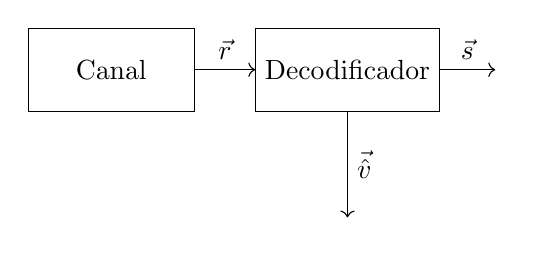
\begin{tikzpicture}[auto, node distance=2cm]

        \node[
            block,
            node distance=3cm,
        ](canal){Canal};

        \node[
            block,
            right of=canal,
            node distance=3cm
        ](deco){Decodificador};

        \node[right of=deco](out){};
        \node[below of=deco](s){};

        \draw[->] (deco) -- node {$\vec{\hat{v}}$} (s);
        \draw[->] (deco) -- node {$\vec{s}$} (out);
        \draw[->] (canal) -- node {$\vec{r}$} (deco);
    \end{tikzpicture}   
\end{center}

El protocolo \textbf{FEC (Forward Error Correction)} corrige los errores en recepción mediante un circuito de detección, en cambio el protocolo \textbf{AQR (Automatic Repeat Request)} manda tramas de control dependiendo de si el mensaje se recibió o no correctamente. En caso de recepción aparentemente correcta ($\vec{s}=\vec{0}$) se responde con una trama de control \textit{ACK}, en caso contrario ($\vec{s}\neq\vec{0}$), se responde con una trama \textit{NACK}.

\subsubsection{Prestaciones técnicas ARQ:}

Teniendo en cuenta que contamos con una transmisión que cumple:

\begin{itemize}
    \item Tráfico unidireccional $E\to R$
    \item Las tramas de control no tinenen errores
    \item $P_{DET_{ERROR}}=\sum_{i=1}^{S}\left(\begin{array}{c}n\\i\end{array}\right)p^i(1-p)^{(n-1)}$
    \item Código bloque lineal $\mathcal{C}(n,k)$
    \item Siempre tenemos datos que transmitir
\end{itemize}

Podemos realizar un análisis de prestaciones técnicas de ARQ calculando la \textbf{cadencia eficaz}, que es la relación entre los bits de informaciín de usuario y el tiempo que está el canal ocupado.

\begin{equation}
    C_{ef} = \frac{K}{T_{oc}}
\end{equation}

\subsubsection{Protocolo de parada y espera}


\begin{figure}[h]
    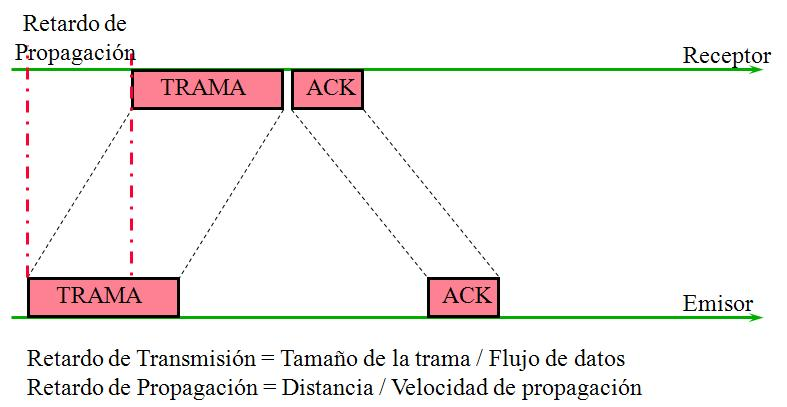
\includegraphics[width=\textwidth]{img/pe.jpeg}
    \caption{Protocolo de parada y espera (origen - Wikipedia)}
\end{figure}


El \textbf{régimen binario $R [\sfrac{bits}{seg}]$} es la capacidad del canal bruta sin tener en cuenta las tramas del control, por lo que el tiempo que se tarda en transmitir los $n$ bits es:

\begin{equation}
    x_p = \frac{n}{R} [seg]
\end{equation}

El \textbf{tiempo de asentimiento $T_{as}$} es el tiempo que tarda el receptor en recibir la información y que el asentimiento sea recibido por el bloque que lo ha enviado. Podemos calcular este tiempo sumando todos los retardos que aportan al canal:

\begin{itemize}
    \item $t_{prop}$ - Tiempo de propagación de los datos
    \item $t_{proc \vec{s}}$ - Tiempo de porcesado del síndrome en recepción
    \item $t_{trans con} = \sfrac{1}{R}$ - Tiempo de transmisión de la trama de control (aproximando como si fuese de longitud 1)
    \item $t_{prop c}$ - Tiempo de propagación de la trama de control
    \item $t_{proc c}$ - Tiempo de procesado de la trama de control
\end{itemize}

Tenemos varias opciones para calcular la cadencia de bits:

\begin{enumerate}
    \item $C_{ef} = \frac{\overline{K}}{\overline{t_{oc}}}$ - como la media de la información y la media del tiempo de ocupación del canal
    \item $C_{ef} = \frac{K}{\overline{t_{oc}}}$ - Fijando el nº de bits de información entre la media de tiempo de ocupación de canal
    \item $C_{ef} = \frac{\overline{K}}{t_{oc}}$ - Fijando el tiempo de ocupación del canal 
\end{enumerate}

La media del tiempo de ocupación $\overline{t_{oc}}$ se calcula de la siguiente forma

\begin{equation}
    \overline{t_{oc}} =
    \sum_{i=1}^{\inf} t_{oc_i}p(i) =
    (x_p+T_{as})\frac{1}{1-P_{RTX}}
\end{equation}

E insertando dentro de la cadencia de bits:

\begin{equation}
    C_{ef} = (1-P_{RTX})\frac{k}{k+m+T_{as}R}R
\end{equation}

Y finalmente, el \textbf{factor de rendimiento} del protocolo de parada y espera es:

\begin{equation}
    \rho = \frac{C_{ef}}{R} = (1-P_{RTX})\frac{k}{k+m+T_{as}R}
\end{equation}

\subsubsection{Envío continuo - Full duplex y rechazo simple}

En este caso, se envían todas las tramas y si se recibe un error, debemos tirar todas las tramas que lleguen hasta que se vuelva a mandar la que toca sin error.

Ahora la cadencia eficaz pasa a ser

\begin{equation}
    C_{ef} = \frac{K}{\overline{T_{oc}}} = (1-P_{RTX})\frac{k}{k+m+T_{as}RP_{RTX}}R
\end{equation}

y la eficacia del canal

\begin{equation}
   \rho = \frac{C_{ef}}{R} = (1-P_{RTX})\frac{k}{k+m+T_{as}RP_{RTX}}
\end{equation}

\subsubsection{Envío continuo y rechazo selectivo}

Este protoco consiste en enviar todos los datos hasta que se recibe un NACK como respuesta, entonces se termina de enviar el paquete que se estaba transmitiendo y se procede a enviar el paquete erróneos.

En este caso, la media del tiempo de ocupación $\overline{t_{oc}}$

\begin{equation}
    \overline{t_{oc}} =
    \frac{k+m}{R}\frac{1}{1-T_{RTX}}
\end{equation}

Y la cadencia eficaz

\begin{equation}
    C_{ef} = \frac{K}{\overline{T_{oc}}} = (1-P_{RTX})\frac{k}{k+m}R
\end{equation}

\subsection{Técnicas hibridas}

\begin{itemize}
    \item \textbf{FEC + FEC:} Consiste en concatenar dos códigos lineares para que el código sea resistente a distintos tipos de errores, por lo que el código se compone de un primer decodificador llamado \textit{codificador externo} y un segundo codificador llamado \textit{codificador interno}, después de la transmisión del canal, el vector recibido pasa priemro por el decodificador interno y después por el externo. El código interno y externo no tienen por que ser del mismo tipo.
    \item \textbf{FEC + ARQ:} Consiste en combinar ambos protocolos para corregir errores pequeños y detectar además de notificar errores de mayor distancia, todo si la distancia el error $d$ entra dentro de la distancia de corrección $t$ o la distancia de detección $d$.
\end{itemize}

\end{document}